%
% A header that lets you compile a chapter by itself, or inside a larger document.
% Adapted from stackoverflow.com/questions/3655454/conditional-import-in-latex
%
%
%Use \inbpdocument and \outbpdocument in your individual files, in place of \begin{document} and \end{document}. In your main file, put in a \def \ismaindoc {} before including or importing anything.
%
% David Duvenaud
% June 2011
% 
% ======================================
%
%


\ifx\ismaindoc\undefined
	\newcommand{\inbpdocument}{
		\def \ismaindoc {}
		% Use this header if we are compiling by ourselves.
		\documentclass[a4paper,11pt,authoryear,index]{common/PhDThesisPSnPDF}
		
%\usepackage{draftwatermark}
%\SetWatermarkLightness{0.95}

% ******************************************************************************
% ****************************** Custom Margin *********************************

% Add `custommargin' in the document class options to use this section
% Set {innerside margin / outerside margin / topmargin / bottom margin}  and
% other page dimensions

\ifsetMargin
\else
    \RequirePackage[left=37mm,right=30mm,top=35mm,bottom=30mm]{geometry}
    \setFancyHdr % To apply fancy header after geometry package is loaded
\fi


%\chead{Unfinished draft}
%\cfoot{\texttt{Unfinished draft - compiled on \today{} at \currenttime}}

% *****************************************************************************
% ******************* Fonts (like different typewriter fonts etc.)*************

% Add `customfont' in the document class option to use this section

\ifsetFont
\else
    % Set your custom font here and use `customfont' in options. Leave empty to
    % load computer modern font (default LaTeX font).  

    \RequirePackage{libertine} 
\fi

% *****************************************************************************
% *************************** Bibliography  and References ********************

%\usepackage{cleveref} %Referencing without need to explicitly state fig /table

% Add `custombib' in the document class option to use this section
\ifsetBib % True, Bibliography option is chosen in class options
\else % If custom bibliography style chosen then load bibstyle here

   \RequirePackage[square, sort, numbers, authoryear]{natbib} % CustomBib

% If you would like to use biblatex for your reference management, as opposed to the default `natbibpackage` pass the option `custombib` in the document class. Comment out the previous line to make sure you don't load the natbib package. Uncomment the following lines and specify the location of references.bib file

% \RequirePackage[backend=biber, style=numeric-comp, citestyle=numeric, sorting=nty, natbib=true]{biblatex}
% \bibliography{References/references} %Location of references.bib only for biblatex

\fi


% changes the default name `Bibliography` -> `References'
\renewcommand{\bibname}{References}


% *****************************************************************************
% *************** Changing the Visual Style of Chapter Headings ***************
% Uncomment the section below. Requires titlesec package.

%\RequirePackage{titlesec}
%\newcommand{\PreContentTitleFormat}{\titleformat{\chapter}[display]{\scshape\Large}
%{\Large\filleft{\chaptertitlename} \Huge\thechapter}
%{1ex}{}
%[\vspace{1ex}\titlerule]}
%\newcommand{\ContentTitleFormat}{\titleformat{\chapter}[display]{\scshape\huge}
%{\Large\filleft{\chaptertitlename} \Huge\thechapter}{1ex}
%{\titlerule\vspace{1ex}\filright}
%[\vspace{1ex}\titlerule]}
%\newcommand{\PostContentTitleFormat}{\PreContentTitleFormat}
%\PreContentTitleFormat


% *****************************************************************************
% **************************** Custom Packages ********************************
% *****************************************************************************


% ************************* Algorithms and Pseudocode **************************

%\usepackage{algpseudocode} 


% ********************Captions and Hyperreferencing / URL **********************

% Captions: This makes captions of figures use a boldfaced small font. 
%\RequirePackage[small,bf]{caption}

\RequirePackage[labelsep=space,tableposition=top]{caption} 
%\renewcommand{\figurename}{Figure} %to support older versions of captions.sty
\captionsetup{labelsep = colon,belowskip=12pt,aboveskip=4pt}

% ************************ Formatting / Footnote *******************************

%\usepackage[perpage]{footmisc} %Range of footnote options 


% ****************************** Line Numbers **********************************

%\RequirePackage{lineno}
%\linenumbers

% ************************** Graphics and figures *****************************

%\usepackage{rotating}
%\usepackage{wrapfig}
%\usepackage{float}
\usepackage{subfig} %note: subfig must be included after the `caption` package. 


% ********************************* Table **************************************

%\usepackage{longtable}
%\usepackage{multicol}
%\usepackage{multirow}
%\usepackage{tabularx}


% ***************************** Math and SI Units ******************************

\usepackage{amsfonts}
\usepackage{amsmath}
\usepackage{amssymb}
%\usepackage{siunitx} % use this package module for SI units


% ******************************************************************************
% ************************* User Defined Commands ******************************
% ******************************************************************************

% *********** To change the name of Table of Contents / LOF and LOT ************

%\renewcommand{\contentsname}{My Table of Contents}
%\renewcommand{\listfigurename}{List of figures}
%\renewcommand{\listtablename}{List of tables}


% ********************** TOC depth and numbering depth *************************

\setcounter{secnumdepth}{2}
\setcounter{tocdepth}{2}

% ******************************* Nomenclature *********************************

% To change the name of the Nomenclature section, uncomment the following line

%\renewcommand{\nomname}{Symbols}


% ********************************* Appendix ***********************************

% The default value of both \appendixtocname and \appendixpagename is `Appendices'. These names can all be changed via: 

%\renewcommand{\appendixtocname}{List of appendices}
%\renewcommand{\appendixname}{Appndx}

		% All my custom preamble stuff.  Shouldn't overlap with anything in official-preamble




% Paths to figure and table directories.
\newcommand{\symmetryfigsdir}{figures/symmetries}
\newcommand{\topologyfiguresdir}{figures/topology}
\newcommand{\infinitefiguresdir}{figures/infinite}
\newcommand{\grammarfiguresdir}{figures/grammar}
\newcommand{\introfigsdir}{figures/intro}
\newcommand{\gplvmfiguresdir}{figures/gplvm}
\newcommand{\warpedfiguresdir}{figures/warped-mixtures}
\newcommand{\deeplimitsfiguresdir}{figures/deep-limits}
\newcommand{\quadraturefigsdir}{figures/quadrature}
\newcommand{\additivefigsdir}{figures/additive}
\newcommand{\decompfigsdir}{figures/decomp}
\newcommand{\examplefigsdir}{figures/worked-example}

\usepackage{bm}  % for warped mixtures - is this necessary?
\usepackage{booktabs}
\usepackage{tabularx}
\usepackage{multirow}
\usepackage{datetime}
\renewcommand{\tabularxcolumn}[1]{>{\arraybackslash}m{#1}}
\usepackage{relsize}
\usepackage{graphicx}
\usepackage{amsmath,amssymb,textcomp}
\usepackage{nicefrac}
\usepackage{amsthm}
\usepackage{tikz}
\usetikzlibrary{arrows}
\usetikzlibrary{calc}
\usepackage{nth}
\usepackage{rotating}
\usepackage{array}
\usepackage{fp}
\usepackage{cleveref}   % Note: this package sometimes causes the page counter to reset.
\crefname{equation}{equation}{equations}
\crefname{figure}{figure}{figures}
%\usepackage{common/sectsty}

% Controls capitalization of all headers
%\usepackage{stringstrings}
%\usepackage[explicit]{titlesec}
%\newcommand\SentenceCase[1]{%
%  \caselower[e]{#1}%
%  \capitalize[q]{\thestring}%
%}
%\titleformat{\section}
%  {\normalfont\Large\bfseries}{\thesection}{1em}{\SentenceCase{#1}\thestring}


%\titleformat{\section} % The normal, unstarred version
%    {\Large\bfseries}{}{2ex}
%    {\thesection. \MakeSentenceCase{#1}}

%\titleformat{name=\section,numberless} % The starred version; note the `numberless` key
%    {\Large\bfseries}{}{2ex}
%    {\MakeSentenceCase{#1}}

\usepackage[hyperpageref]{backref}
% Setup to show (pages 4 and 9) sort of thing in the bibliography - DD
%\def\foo{\hspace{\fill}\mbox{}\linebreak[0]\hspace*{\fill}}
%\def\foo{\parbox{3cm}{\hfill}
%\def\foo{\parbox{3cm}{\hfill}
%\newcommand\foo[1]{{\raggedleft{\hfill{\mbox{\hfill{#1}}}}}}
\newcommand{\comfyfill}[1]{% = Thorsten Donig's \signed
  \unskip\hspace*{0.1em plus 1fill}
  \nolinebreak[3]%
  \hspace*{\fill}\mbox{#1}
  \parfillskip0pt\par
}
\newcommand\foo[1]{{\comfyfill{\mbox{#1}}}}
%\newcommand\foo[1]{{\mbox{#1}}}
\renewcommand*{\backref}[1]{}
\renewcommand*{\backrefalt}[4]{%
\ifcase #1 %
%
\or
\foo{(page #2)}%
\else
\foo{(pages #2)}%
\fi
}

\usepackage{stringstrings}

%\newcommand{\headercase}{\
%\DeclareFieldFormat{titlecase}{\MakeSentenceCase{#1}}


%% For submission, make all render blank.
%%%%%%%%%%%%%%%%%%%%%%%%%%%%%%%%%%%%%%%%%%%%%%%%%%%%%%%%%%
%%%% EDITING HELPER FUNCTIONS  %%%%%%%%%%%%%%%%%%%%%%%%%%%
%%%%%%%%%%%%%%%%%%%%%%%%%%%%%%%%%%%%%%%%%%%%%%%%%%%%%%%%%%

%% NA: needs attention (rough writing whose correctness needs to be verified)
%% TBD: instructions for how to fix a gap ("Describe the propagation by ...")
%% PROBLEM: bug or missing crucial bit 

%% use \fXXX versions of these macros to put additional explanation into a footnote.  
%% The idea is that we don't want to interrupt the flow of the paper or make it 
%% impossible to read because there are a bunch of comments.

%% NA's (and TBDs, those less crucially) should be written so 
%% that they flow with the text.

\definecolor{WowColor}{rgb}{.75,0,.75}
\definecolor{SubtleColor}{rgb}{0,0,.50}

% inline
\newcommand{\NA}[1]{\textcolor{SubtleColor}{ {\tiny \bf ($\star$)} #1}}
\newcommand{\LATER}[1]{\textcolor{SubtleColor}{ {\tiny \bf ($\dagger$)} #1}}
\newcommand{\TBD}[1]{\textcolor{SubtleColor}{ {\tiny \bf (!)} #1}}
\newcommand{\PROBLEM}[1]{\textcolor{WowColor}{ {\bf (!!)} {\bf #1}}}

% as margin notes

\newcounter{margincounter}
\newcommand{\displaycounter}{{\arabic{margincounter}}}
\newcommand{\incdisplaycounter}{{\stepcounter{margincounter}\arabic{margincounter}}}

\newcommand{\fTBD}[1]{\textcolor{SubtleColor}{$\,^{(\incdisplaycounter)}$}\marginpar{\tiny\textcolor{SubtleColor}{ {\tiny $(\displaycounter)$} #1}}}

\newcommand{\fPROBLEM}[1]{\textcolor{WowColor}{$\,^{((\incdisplaycounter))}$}\marginpar{\tiny\textcolor{WowColor}{ {\bf $\mathbf{((\displaycounter))}$} {\bf #1}}}}

\newcommand{\fLATER}[1]{\textcolor{SubtleColor}{$\,^{(\incdisplaycounter\dagger)}$}\marginpar{\tiny\textcolor{SubtleColor}{ {\tiny $(\displaycounter\dagger)$} #1}}}

%\renewcommand{\LATER}[1]{}
%\renewcommand{\fLATER}[1]{}
%\renewcommand{\TBD}[1]{}
%\renewcommand{\fTBD}[1]{}
%\renewcommand{\PROBLEM}[1]{}
%\renewcommand{\fPROBLEM}[1]{}
%\renewcommand{\NA}[1]{}


% HUMBLE WORDS: shown slightly smaller when in normal text
% Thanks to Christian Steinruecken!

% HUMBLE WORDS: shown slightly smaller when in normal text
% Christian Steinruecken
%
\makeatletter%
%\def\@humbleformat#1{{\fontsize{}{1em}\selectfont #1}}
%\def\@humbleformat#1{\textsmaller{#1}}%
\newlength{\nonHumbleHeight}
\def\@humbleformat#1{{\settoheight{\nonHumbleHeight}{#1}\resizebox{!}{0.94\nonHumbleHeight}{#1}}}%
\def\@idxhumbleformat#1{{\relscale{0.95}{#1}}}%
%\def\@humbleformat#1{{#1}}%
\def\declareHumble#1#2{%
  \expandafter\def\csname #1\endcsname{\@humbleformat{#2}}%
  \expandafter\def\csname s#1\endcsname{{#2}}%
  \expandafter\def\csname idx#1\endcsname{{\@idxhumbleformat{#2}}}%
}%
\def\humble#1{\@humbleformat{#1}}%
\def\idxhumble#1{\@idxhumbleformat{#1}}%
\makeatother%

% Convenient indexing for humble abbreviations
\def\humbleindex#1#2{\index{#1@\idxhumble{#1}}}



% TODO: Clean up duplicates
\declareHumble{ANOVA}{ANOVA}
\declareHumble{ARD}{ARD}
\declareHumble{BIC}{BIC}
\declareHumble{BMC}{BMC}
\declareHumble{bq}{BQ}
\declareHumble{CRP}{CRP}
\declareHumble{dirpro}{DP}
\declareHumble{HDMR}{HDMR}
\declareHumble{GAM}{GAM}
\declareHumble{GEM}{GEM}
\declareHumble{GMM}{GMM}
\declareHumble{gplvm}{GP-LVM}
\declareHumble{gpml}{GPML}
\declareHumble{GPML}{GPML}
\declareHumble{gprn}{GPRN}
\declareHumble{gpt}{GP}
\declareHumble{gp}{GP}
\declareHumble{HKL}{HKL}
\declareHumble{HMC}{HMC}
\declareHumble{ibp}{IBP}
\declareHumble{iGMM}{iGMM}
\declareHumble{iwmm}{iWMM}
\declareHumble{kCP}{CP}
\declareHumble{kCW}{CW}
\declareHumble{kC}{C}
\declareHumble{KDE}{KDE}
\declareHumble{kLin}{Lin}
\declareHumble{KPCA}{KPCA}
\declareHumble{kPer}{Per}
\declareHumble{kPerGen}{ZMPer}
\declareHumble{kRQ}{RQ}
\declareHumble{kSE}{SE}
\declareHumble{kWN}{WN}
\declareHumble{Lin}{Lin}
\declareHumble{LBFGS}{L-BFGS}
\declareHumble{LIBSVM}{LIBSVM}
\declareHumble{MAP}{MAP}
\declareHumble{mcmc}{MCMC}
\declareHumble{MKL}{MKL}
\declareHumble{MLP}{MLP}
\declareHumble{MNIST}{MNIST}
\declareHumble{MSE}{MSE}
\declareHumble{OU}{OU}
\declareHumble{Per}{Per}
\declareHumble{RBF}{RBF}
\declareHumble{RMSE}{RMSE}
\declareHumble{RQ}{RQ}
\declareHumble{SBQ}{SBQ}
\declareHumble{seard}{SE-ARD}
\declareHumble{sefull}{SE-\textnormal{full}}
\declareHumble{SEGP}{SE-GP}
\declareHumble{SE}{SE}
\declareHumble{SNR}{SNR}
\declareHumble{SSANOVA}{SS-ANOVA}
\declareHumble{SVM}{SVM}
\declareHumble{UCI}{UCI}
\declareHumble{UMIST}{UMIST}
\declareHumble{vbgplvm}{VB GP-LVM}

\newcommand{\kSig}{\boldsymbol\sigma}

\def\subexpr{{\cal S}}
\def\baseker{{\cal B}}
\def\numWinners{k}

\def\ie{i.e.\ }
\def\eg{e.g.\ }
\def\etc{etc.\ }
\let\oldemptyset\emptyset
%\let\emptyset 0




% Unify notation between neural-net land and GP-land.
\newcommand{\hphi}{h}
\newcommand{\hPhi}{\vh}
\newcommand{\walpha}{w}
\newcommand{\wboldalpha}{\bw}
\newcommand{\wcapalpha}{\vW}
\newcommand{\lengthscale}{w}

\newcommand{\layerindex}{\ell}



\newcommand{\gpdrawbox}[1]{
\setlength\fboxsep{0pt}
\hspace{-0.15in} 
\fbox{
\includegraphics[width=0.464\columnwidth]{\deeplimitsfiguresdir/deep_draws/deep_gp_sample_layer_#1}
}}



\newcommand{\procedurename}{ABCD}
\newcommand{\genText}[1]{{\sf #1}}



\newcommand{\asdf}{$^{\textnormal{th}}$}

\newcommand{\binarysum}{\sum_{\bf{x} \in \{0,1\}^D}}
\newcommand{\expect}{\mathbb{E}}
\newcommand{\expectargs}[2]{\mathbb{E}_{#1} \left[ {#2} \right]}
\newcommand{\var}{\mathbb{V}}
\newcommand{\varianceargs}[2]{\mathbb{V}_{#1} \left[ {#2} \right]}
\newcommand{\cov}{\operatorname{cov}}
\newcommand{\Cov}{\operatorname{Cov}}
\newcommand{\covargs}[2]{\Cov \left[ {#1}, {#2} \right]}
\newcommand{\variance}{\mathbb{V}}
\newcommand{\vecop}[1]{\operatorname{vec} \left( {#1} \right)}

\newcommand{\covarianceargs}[2]{\Cov_{#1} \left[ {#2} \right]}
\newcommand{\colvec}[2]{\left[ \begin{array}{c} {#1} \\ {#2} \end{array} \right]}
\newcommand{\tbtmat}[4]{\left[ \begin{array}{cc} {#1} & {#2} \\ {#3} & {#4} \end{array} \right]}

\newcommand{\acro}[1]{{\humble{#1}}}
%\newcommand{\vect}[1]{\boldsymbol{#1}}
\newcommand{\vect}[1]{{\bf{#1}}}
\newcommand{\mat}[1]{\mathbf{#1}}
\newcommand{\pderiv}[2]{\frac{\partial #1}{\partial #2}}
\newcommand{\npderiv}[2]{\nicefrac{\partial #1}{\partial #2}}

\newcommand{\pha}{^{\phantom{:}}}

\newcommand{\argmin}{\operatornamewithlimits{argmin}}
\newcommand{\argmax}{\operatornamewithlimits{argmax}}

% The following designed for probabilities with long arguments

\newcommand{\Prob}[2]{P\!\left(\,#1\;\middle\vert\;#2\,\right)}
\newcommand{\ProbF}[3]{P\!\left(\,#1\!=\!#2\;\middle\vert\;#3\,\right)}
\newcommand{\p}[2]{p\!\left(#1\middle\vert#2\right)}
\newcommand{\po}[1]{p\!\left(#1\right)}
\newcommand{\pF}[3]{p\!\left(\,#1\!=\!#2\;\middle\vert\;#3\,\right)} 
\newcommand{\mean}[2]{{m}\!\left(#1\middle\vert#2\right)}



\newcommand{\valpha}{\boldsymbol{\alpha}}
\newcommand{\va}{\vect{a}}
\newcommand{\vA}{\vect{A}}
\newcommand{\vB}{\mat{B}}
\newcommand{\vb}{\vect{b}}
\newcommand{\vC}{\mat{C}}
\newcommand{\vc}{\vect{c}}
\newcommand{\vecf}{\boldsymbol{f}}
\newcommand{\vell}{\vect{\ell}}
\newcommand{\vepsilon}{\boldsymbol{\epsilon}}
\newcommand{\veps}{\boldsymbol{\epsilon}}
\newcommand{\ve}{\boldsymbol{\epsilon}}
\newcommand{\vf}{\vecf}
\newcommand{\vg}{\vect{g}}
\newcommand{\vh}{\vect{h}}
\newcommand{\vI}{\mat{I}}
\newcommand{\vK}{\mat{K}}
\newcommand{\vk}{\vect{k}}
\newcommand{\vL}{\mat{L}}
\newcommand{\vl}{\vect{l}}
\newcommand{\vmu}{{\boldsymbol{\mu}}}
\newcommand{\vone}{\vect{1}}
\newcommand{\vphi}{{\boldsymbol{\phi}}}
\newcommand{\vpi}{{\boldsymbol{\pi}}}
\newcommand{\vq}{\vect{q}}
\newcommand{\vR}{\mat{R}}
\newcommand{\vr}{\vect{r}}
\newcommand{\vsigma}{{\boldsymbol{\sigma}}}
\newcommand{\vSigma}{\mat{\Sigma}}
\newcommand{\vS}{\mat{S}}
\newcommand{\vs}{\vect{s}}
\newcommand{\vtheta}{{\boldsymbol{\theta}}}
\newcommand{\vu}{\vect{u}}
\newcommand{\vV}{\mat{V}}
\newcommand{\vW}{\mat{W}}
\newcommand{\vw}{\vect{w}}
\newcommand{\vX}{\mat{X}}
\newcommand{\vx}{\vect{x}}
\newcommand{\vY}{\mat{Y}}
\newcommand{\vy}{\vect{y}}
\newcommand{\vzero}{\vect{0}}
\newcommand{\vZ}{\mat{Z}}
\newcommand{\vz}{\vect{z}}


% deep gp notation
\newcommand{\netweights}{w}
\newcommand{\vnetweights}{\vw}
\newcommand{\mnetweights}{\vW}
\newcommand{\outweights}{\v}
\newcommand{\voutweights}{\vv}
\newcommand{\moutweights}{\vV}

\newcommand{\unitparams}{\v}
\newcommand{\vunitparams}{\vv}
\newcommand{\munitparams}{\vV}


\newcommand{\He}{\mathcal{H}}
\newcommand{\normx}[2]{\left\|#1\right\|_{#2}}
\newcommand{\Hnorm}[1]{\normx{#1}{\He}}
\newcommand{\mmd}{{\rm MMD}}


\newcommand{\mf}{\bar{\vf}}

%\newcommand{\mf}{\mu} %{\bar{\ell}}
\newcommand{\lf}{f} % Likelihood function
\newcommand{\st}{_\star}

% from simpler log-bq writeup
\newcommand{\lftwo}{{\log \ell}}
\newcommand{\mftwo}{{\bar \ell}}
\newcommand{\loggp}{{\log\acro{GP}}}%| \bX, \vy )}}
\newcommand{\loggpdist}{{\acro{GP}(\lftwo)}}%| \vX, \vy )}}


\newcommand{\inv}{^{{\mathsmaller{-1}}}}
\newcommand{\tohalf}{^{{\mathsmaller{\nicefrac{1}{2}}}}}

\newcommand{\Normal}{\mathcal{N}}
\newcommand{\N}[3]{\mathcal{N}\!\left(#1 \middle| #2,#3\right)}
\newcommand{\Nt}[2]{\mathcal{N}\!\left(#1,#2\right)}
\newcommand{\NT}[2]{\mathcal{N}\!\left(#1,#2\right)}
\newcommand{\GPdist}[3]{\mathcal{GP}\!\left(#1 \, \middle| \, #2, #3 \right)}
\newcommand{\GPdisttwo}[2]{\mathcal{GP}\!\left(\, #1, #2 \right)}
\newcommand{\bN}[3]{\mathcal{N}\big(#1 \middle| #2,#3\big)}
\newcommand{\boldN}[3]{\text{\textbf{\mathcal{N}}}\big(#1;#2,#3\big)}
\newcommand{\ones}[1]{\mat{1}_{#1}}
\newcommand{\eye}[1]{\mat{E}_{#1}}
\newcommand{\tra}{^{\mathsf{T}}}
%\newcommand{\tra}{^{\top}}
%\mathsf{T}
\newcommand{\trace}{\operatorname{tr}}
\newcommand{\shift}{\operatorname{shift}}
\renewcommand{\mod}{\operatorname{mod}}
\newcommand{\deq}{:=}
\newcommand{\oneofk}{\operatorname{one-of-k}}
%\newcommand{\degree}{^\circ}

\newcommand{\GPt}[2]{\mathcal{GP}\!\left(#1,#2\right)}
%\newcommand{\GPt}[2]{\gp\!\left(#1,#2\right)}

\DeclareMathOperator{\tr}{tr}
\DeclareMathOperator{\chol}{chol}
\DeclareMathOperator{\diag}{diag}

\newenvironment{narrow}[2]{%
  \begin{list}{}{%
  \setlength{\topsep}{0pt}%
  \setlength{\leftmargin}{#1}%
  \setlength{\rightmargin}{#2}%
  \setlength{\listparindent}{\parindent}%
  \setlength{\itemindent}{\parindent}%
  \setlength{\parsep}{\parskip}}%
\item[]}{\end{list}}



\newcommand{\dist}{\ \sim\ }
\def\given{\,|\,}

% Table stuff
\newcolumntype{C}[1]{>{\centering\let\newline\\\arraybackslash\hspace{0pt}}m{#1}}
\newcolumntype{L}[1]{>{\raggedright\let\newline\\\arraybackslash\hspace{0pt}}m{#1}}
\newcolumntype{R}[1]{>{\raggedleft\let\newline\\\arraybackslash\hspace{0pt}}m{#1}}

\newcommand{\defeq}{\mathrel{:\mkern-0.25mu=}}

\def\ie{i.e.\ }
\def\eg{e.g.\ }
\def\iid{i.i.d.\ }
%\def\simiid{\sim_{\mbox{\tiny iid}}}
\def\simiid{\overset{\mbox{\tiny iid}}{\sim}}
\def\simind{\overset{\mbox{\tiny \textnormal{ind}}}{\sim}}
\def\eqdist{\stackrel{\mbox{\tiny d}}{=}}
%\newcommand{\distas}[1]{\mathbin{\overset{#1}{\kern \z@ \sim}}}
%TODO: fix this - it worked outside the thesis!
\newcommand{\distas}[1]{\mathbin{\overset{#1}{\sim}}}

\def\Reals{\mathbb{R}}

\def\Uniform{\mbox{\rm Uniform}}
\def\Bernoulli{\mbox{\rm Bernoulli}}
\def\GP{\mathcal{GP}}
\def\GPLVM{\mathcal{GP-LVM}}




% Kernel stuff

\def\iva{\vect{\inputVar}}
\def\ivaone{\inputVar}
\def\inputVar{x}
\def\InputVar{X}
\def\InputSpace{\mathcal{X}}
\def\outputVar{y}
\def\OutputSpace{\mathcal{Y}}
\def\function{f}
\def\kernel{k}
\def\KernelMatrix{K}
\def\SumKernel{\sum}
\def\ProductKernel{\prod}
\def\expression{e}
\def\feat{\vh}

\newcommand{\kerntimes}{ \! \times \!}
\newcommand{\kernplus}{ \, + \,}


% Proof stuff
\theoremstyle{plain}
\newtheorem{theorem}{Theorem}[section]
\newtheorem{lemma}[theorem]{Lemma}
\newtheorem{prop}[theorem]{Proposition}
\newtheorem{proposition}{Proposition}
\newtheorem*{cor}{Corollary}

% For infinite bq
\newcommand{\iv}{\theta}
\newcommand{\viv}{\vtheta}

% For intro chapter
\newcommand{\funcval}{\vf(\vX)}
\newcommand{\testpoint}{{\vx^\star}}

\newcommand{\underwrite}[2]{{\underbrace{#1}_{\textnormal{#2}}}}



% For kernel figures
\newcommand{\fhbig}{2cm}%
\newcommand{\fwbig}{3cm}%
\newcommand{\kernpic}[1]{\includegraphics[height=\fhbig,width=\fwbig]{\grammarfiguresdir/structure_examples/#1}}%
\newcommand{\kernpicr}[1]{\rotatebox{90}{\includegraphics[height=\fwbig,width=\fhbig]{\grammarfiguresdir/structure_examples/#1}}}%
\newcommand{\addkernpic}[1]{{\includegraphics[height=\fhbig,width=\fwbig]{\grammarfiguresdir/additive_multi_d/#1}}}%
\newcommand{\largeplus}{\tabbox{{\Large+}}}%
\newcommand{\largeeq}{\tabbox{{\Large=}}}%
\newcommand{\largetimes}{\tabbox{{\Large$\times$}}}%
\newcommand{\fixedx}{$x$ (with $x' = 1$)}%

% for warped mixtures
\newcommand{\CLAS}{\vz}  %cluster assignments
\newcommand{\CLASi}{z} % individual cluster assignments


		% ************************ Thesis Information & Meta-data **********************

%% The title of the thesis
\title{Automating statistical modelling}

%\texorpdfstring is used for PDF metadata. Usage:
%\texorpdfstring{LaTeX_Version}{PDF Version (non-latex)} eg.,
%\texorpdfstring{$sigma$}{sigma}

%% The full name of the author
\author{James Robert Lloyd}

%% Department (eg. Department of Engineering, Maths, Physics)
%\dept{Department of Engineering}

%% University and Crest
\university{University of Cambridge}
\crest{
\includegraphics[width=0.25\textwidth]{misc/University_Crest}}

%% You can redefine the submission text:
% Default as per the University guidelines: This dissertation is submitted for
% the degree of Doctor of Philosophy
%\renewcommand{\submissiontext}{change the default text here if needed}

%% Full title of the Degree 
\degree{Doctor of Philosophy}
 
%% College affiliation (optional)
\college{Trinity College}

%% Submission date
\degreedate{December 2014} 

%% Meta information
\subject{Machine Learning}
\keywords{{LaTeX} {PhD Thesis} {Engineering} {University of Cambridge} {Machine Learning} {Gaussian processes} {Time Series} {Model checking} {Model criticism} {Aldous--Hoover} {Networks}}



		\begin{document}
	}	
	\newcommand{\outbpdocument}[1]{
		% Fake chapters so references aren't broken
		\label{ch:intro}                
		\label{ch:dummy}
		\label{ch:discussion}
		%\bibliographystyle{common/CUEDthesis}
		\bibliographystyle{plainnat}
		\bibliography{references.bib}
		\end{document}
	}	
\else
	%If we're inside another document, no need to re-start the document.
	\ifx\inbpdocument\undefined
		\newcommand{\inbpdocument}{}
		\newcommand{\outbpdocument}[1]{}
	\fi
\fi

\inbpdocument

\chapter{A method to determine where a statistical model is most wrong}
\label{ch:criticism}

The automatic statistical reports that were the output of the work of chapter~\ref{ch:description} all conclude with a model criticism section.
In this section, the statistical model presented to the user is presented as a scientific hypothesis and as such it subjected to attempts to falsify its claims.
On entering the literature of statistical model criticism I quickly found myself in the cross fire of a version of the frequentists versus Bayesians argument which appears to have been left unresolved.
Moreover, I have found there to be little actionable advice on which methods of model criticism to use when, which presented a challenge when trying to select appropriate model criticism methods to be used by a system capable of constructing infinitely many different statistical models.

This chapter is my initial response to these gaps in the literature.
My own opinion on the correct philosophy for model criticism is still in flux so I will discuss emerging ideas at the end of this chapter.

\section{Introduction}

Statistical model checking or criticism\footnotemark{} is an important part of a complete statistical analysis.
\footnotetext{We follow Box \citep{Box1980-ud} using the term `model criticism' for similar reasons to O'Hagan \citep{OHagan2003-bc}.}
When one fits a linear model to a data set via least squares a complete analysis includes computing \eg Cook's distances \cite{Cook1982-eq} to identify influential points or plotting residuals against fitted values to identify non-linearity or heteroscedasticity.
Similarly, modern approaches to Bayesian statistics view model criticism as in important component of an iterative cycle of model construction, inference and criticism \citep{Gelman2013-st}.

As statistical models become more complex and diverse in response to the challenges of modern data sets there will be an increasing need for a greater range of model criticism procedures that are either automatic or generally applicable.
This will be especially true as automatic modelling methods \citep[e.g.][]{Grosse2012-zf, Thornton2013-zg, Lloyd2014-ABCD} and probabilistic programming \citep[e.g.][]{Milch2007-dz, Goodman2012-pf, stan-software:2014} mature\fTBD{What is the canonical 1997 reference?}.

Model criticism typically proceeds by choosing a statistic of interest, computing it on data and comparing this to a suitable null distribution.
Ideally these statistics are chosen to assess the utility of the statistical model under consideration (see applied examples \citep[e.g.][]{Meulders1998-xo, Gelman2013-st}) but this can require considerable expertise on the part of the modeller.
We propose an alternative to this approach by using a statistic defined as a supremum over a broad class of measures of discrepancy between two distributions, the maximum mean discrepancy (MMD) \citep[e.g.][]{Borgwardt2006-gy, Gretton2007-ft, Gretton2008-ik}).
The advantage of this approach is that the discrepancy measure attaining the supremum automatically identifies regions of the data which are most poorly represented by the statistical model fit to the data.

We demonstrate this approach to model criticism on toy data sets, restricted Boltzmann machines\fTBD{what is a canonical reference?} and deep belief networks\fTBD{what is a canonical reference?} trained on MNIST digits and Gaussian process \citep[e.g.][]{Rasmussen2006-ml} regression models trained on several time series.
Our proposed method identifies discrepancies between the data and fitted models that would not be apparent from the predictive performance focused metrics one typically finds in a machine learning paper\fTBD{Should we be explicitly referring to machine learning}.
It is our belief\fTBD{I'm finding it difficult to find the right words here} that more effort shoud be expended on attempting to falsify models fitted to data, using model criticism techniques or otherwise.
Not only will this aid research in targeting areas for improvement but it should give greater confidence in any conclusions drawn from a model.

\section{Model criticism}
\label{sec:model-crit-general}

Suppose we observe data $Y^\textrm{obs} = (y_i)_{i=1\ldots n}$ and we attempt to fit a model $M$ with parameters $\theta$.
After performing a statistical analysis we will have either an estimate, $\hat\theta$, or an (approximate) posterior, $p(\theta \given Y^\textrm{obs}, M)$, for the parameters.
How can we check the validity of this analysis?

\subsection{Criticising prior assumptions}

The classical approach to model criticism is to attempt to falsify the null hypothesis that the data could have been generated by the model $M$ for some value of the parameters $\theta$ \ie ${Y^\textrm{obs} \sim p(Y \given \theta, M)}$.
This is typically achieved by constructing a statistic $T$ of the data whose distribution does not depend on the parameters $\theta$ \ie a pivotal quantity.
The extent to which the observed data $Y^\textrm{obs}$ differs from expectations under the model $M$ could then be quantified with a tail-area based $p$-value
\begin{equation}
  p_\textrm{freq}(Y^\textrm{obs}) = \mathbb{P}(T(Y)\geq T(Y^\textrm{obs})) \quad \textrm{where} \quad Y \sim p(Y \given \theta, M) \quad \textrm{for any } \theta.
  \label{eq:freq-p-value}
\end{equation}

Analogous quantities in a Bayesian analysis are the prior predictive $p$-values of Box \citep{Box1980-ud}.
The null hypothesis is replaced with the claim that the data could have been generated from the prior predictive distribution ${Y^\textrm{obs} \sim \int p(Y \given \theta, M)p(\theta \given M) \mathrm{d}\theta}$.
A tail-area $p$-value can then be constructed for any statistic $T$ of the data
\begin{equation}
  p_\textrm{prior}(Y^\textrm{obs}) = \mathbb{P}(T(Y)\geq T(Y^\textrm{obs})) \quad \textrm{where} \quad Y \sim \int p(Y \given \theta, M)p(\theta \given M) \mathrm{d}\theta.
  \label{eq:prior-p-value}
\end{equation}

Both of these procedures construct a function of the data $p(Y^\textrm{obs})$ whose distribution under a suitable null hypothesis is uniform \ie a $p$-value.
The $p$-value quantifies how surprised one should be after observing data $Y^\textrm{obs}$ having expected it to have been generated by the model.
The different null hypotheses reflect the different uses of the word `model' in frequentist and Bayesian analyses.
A frequentist model is a class of probability distributions over data indexed by parameters whereas a Bayesian model is a joint probability distribution over data and parameters.

\subsection{Criticising estimated models or posterior distributions}

A constrasting method of Bayesian model criticism is the calculation of posterior predictive $p$-values \citep[e.g.][]{Guttman1967-my, Rubin1984-tw} $p_\textrm{post}$ where the prior predictive distribution is replaced with the posterior predictive distribution ${Y \sim \int p(Y \given \theta, M)p(\theta \given Y^\textrm{obs}, M) \mathrm{d}\theta}$.
The corresponding test for an analysis resulting in a point estimate of the parameters $\hat\theta$ would use the plug-in predictive distribution ${Y \sim p(Y \given \hat\theta, M)}$ to form the plug-in $p$-value $p_\textrm{plug}$.

These $p$-values quantify how surprised one should be if, after performing inference having observed data $Y^\textrm{obs}$, one were to observe new data whose value of the statistic $T$ was equal to that of the original data.
Put more simply, they quantify how surprising the data $Y^\textrm{obs}$ is even after having observed it.
A simple variant of this method of model criticism is to use held out data $Y^*$, generated from the same distribution as $Y^\textrm{obs}$, to compute a $p$-value \ie ${p(Y^*) = \mathbb{P}(T(Y)\geq T(Y^*))}$.
This quantifies how surprising the held out data is after having observed $Y^\textrm{obs}$.

\subsection{Which type of model criticism should be used?}

Different forms of model criticism are appropriate in different contexts, but we believe that posterior predictive and plug-in $p$-values will be most often useful for the types of statistical model considered in the machine learning literature.
For example, suppose one is fitting a nonparametric or otherwise very flexible model to data \eg a deep belief network.
Classical $p$-values would assume a null hypothesis that the data could have been generated from some deep belief network.
Since the space of all possible deep belief networks is very large it will be difficult to ever falsify this hypothesis.
A more interesting null hypothesis to test in this example is whether or not our particular deep belief network can faithfully mimick the distribution it was trained on.
This is the null hypothesis of posterior or plug-in $p$-values.

\section{Model criticism for \iid data using two sample tests}
\label{sec:model-crit-two-sample}

We assume that our data $Y$ are \iid samples from some unknown distribution ${(y_i)_{i=1\ldots n} \simiid p(y\given \theta, M)}$.
After performing inference resulting in a point estimate of the parameters $\hat\theta$, the null hypothesis associated with a plug-in $p$-value is ${(y^\textrm{obs}_i)_{i=1\ldots n} \simiid p(y \given \hat\theta, M)}$.

We can test this null hypothesis using a two sample test \citep[e.g.][]{Friedman1979-ur, Bickel1969-ao, Hotelling1951-jd}.
In particular, we have samples of data $(y_i)_{i=1\ldots n}$ and we can generate samples from the plug-in predictive distribution ${(y_i^\textrm{rep})_{i=1\ldots m} \simiid p(y \given \hat\theta, M)}$ and then test whether or not these samples could have been generated from the same distribution.

The methods for constructing $p$-values in the previous section all started with a statistic $T$ of the entire data.
This however is not necessary; a $p$-value is simply a random variable which has a uniform distribution under the null hypothesis.
Instead of computing a statistic $T(Y^\textrm{obs})$ of the entire data we consider statistics of data points $t(y)$ and then consider the mean discrepancy between the two samples
\begin{equation}
\mathbb{E}(t(y^\textrm{rep})) - \mathbb{E}(t(y)).
\end{equation}

This quantity measures how different the two distributions are on average as measured by the statistic $t$.
The benefit of mean discrepancy measures is that we can analytically maximise the discrepancy over a large class of statistics $t$, allowing us to find the statistic that most shows any discrepancy between the two distributions.

\section{Kernel maximum mean discrepancy (MMD) two sample tests}

Consider the two sample problem. We are given samples ${X = (x_i)_{i=1\ldots m}}$ and ${Y = (y_i)_{i=1\ldots n}}$ drawn \iid from distributions $p$ and $q$ respectively.
Can we determine if $p \neq q$?

An answer to this problem is to consider maximum mean discrepancy (MMD) \citep{Gretton2008-ik} statistics (also called integral probability metrics \citep{Muller1997-vs})
\begin{equation}
\textrm{MMD}(\mathcal{F},p,q) = \sup_{f \in \mathcal{F}}(\mathbb{E}_{x\sim p}[f(x)] - \mathbb{E}_{y\sim q}[f(y)])
\label{eq:MMD}
\end{equation}
where $\mathcal{F}$ is a set of functions.
When $\mathcal{F}$ is a reproducing kernel Hilbert space (RKHS) the function attaining the supremum can be derived analytically and is called the witness function
\begin{equation}
f(x) = \mathbb{E}_{x'\sim p}[k(x,x')] - \mathbb{E}_{x'\sim q}[k(x,x')]
\label{eq:witness}
\end{equation}
where $k$ is the kernel of the RKHS.

Substituting this expression into equation~\eqref{eq:MMD} yields
\begin{equation}
  \textrm{MMD}^2(\mathcal{F},p,q) = \mathbb{E}_{x,x'\sim p}[k(x,x')] + 2\mathbb{E}_{x\sim p,y\sim q}[k(x,y)] + \mathbb{E}_{y,y'\sim q}[k(y,y')].
\end{equation}

This expression only involves expectations of the kernel $k$ which can be estimated empirically by
%\end{eqnarray}
\begin{equation}
  \textrm{MMD}_b^2(\mathcal{F},X,Y) = \frac{1}{m^2}\sum_{i,j=1}^{m}k(x_i,x_j) - \frac{2}{mn}\sum_{i,j=1}^{m,n}k(x_i,y_j) + \frac{1}{n^2}\sum_{i,j=1}^{n}k(y_i,y_j).
\label{eq:MMD_b}
\end{equation}

One can also estimate the witness function from finite samples
\begin{equation}
\hat{f}(x) = \frac{1}{m}\sum_{i=1}^{m}k(x,x_i) - \frac{1}{n}\sum_{i=1}^{n}k(x,y_i)
\label{eq:witness-estimate}
\end{equation}
\ie the empirical witness function is the difference of two kernel density estimates \citep[e.g.][]{Rosenblatt1956-hx, Parzen1962-hk}.
This means that we can interpret the witness function as showing where the estimated densities of $p$ and $q$ are most different.

\subsection{Kernel choice}

The nature of the two sample test defined by the kernel MMD depends on the choice of the kernel.
In this paper we use the radial basis function kernel, also known as the squared exponential or exponentiated quadratic.
This kernel encodes for smooth functions characterised by a typical lengthscale \citep[e.g.][]{Rasmussen2006-ml}.
A typical heuristic for selecting the lengthscale is to use the median distance between all points as the lengthscale \citep[e.g.][]{Gretton2008-ik}.
However, since we interpret the witness function as the difference of two kernel density estimates we also consider selecting the lengthscale which gives the best density estimates (see section~\ref{sec:high_dim}).

\subsection{Estimation of the null distribution}

There are a number of different ways in which the null distribution of the MMD statistic~\eqref{eq:MMD_b} can be estimated \citep[e.g.][]{Gretton2008-ik}.
We use the bootstrap variant for its simplicity and general applicability.
Note that the MMD two sample test using the bootstrap estimation of the null distribution is an example of a permutation test \TBD{reference something}.

\section{Examples on toy data}

\subsection{Newcomb's speed of light data}

A histogram of Simon Newcomb's 66 measurements used to determine the speed of light \citep{Stigler1977-dd} is shown on the left of figure~\ref{fig:newcomb}.
We consider fitting a normal distribution to this data by maximum likelihood.

\begin{figure}[ht]
\centering
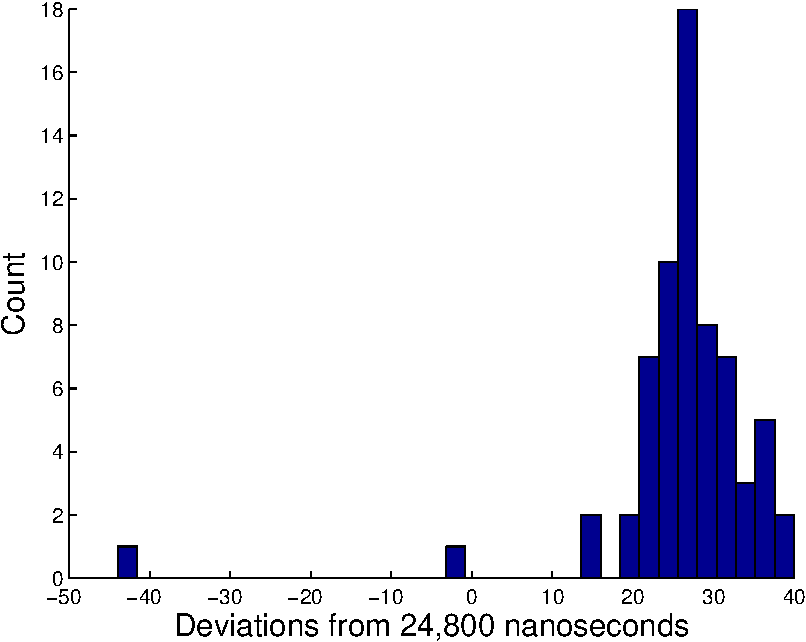
\includegraphics[width=0.29\columnwidth]{\criticismfigsdir/newcomb_hist}
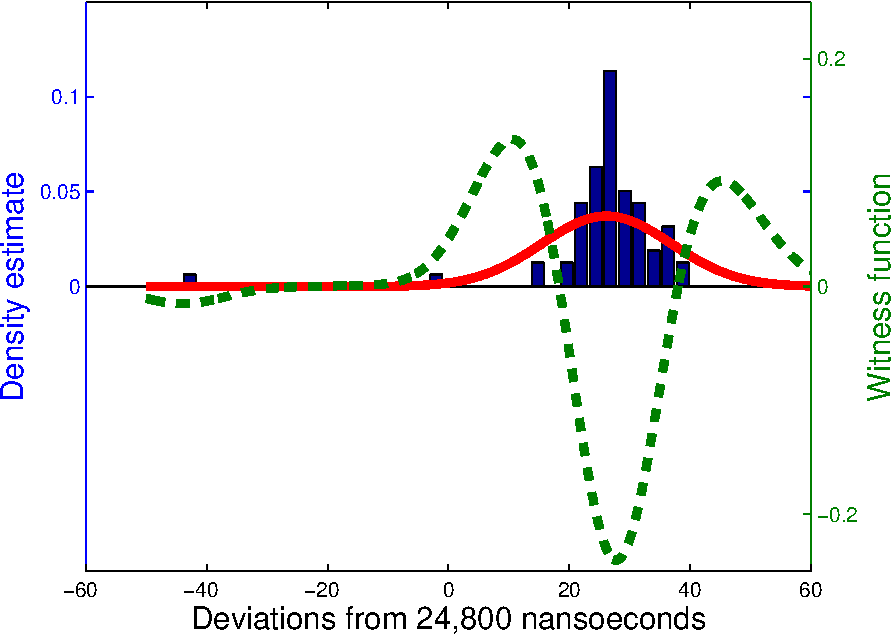
\includegraphics[width=0.32\columnwidth]{\criticismfigsdir/newcomb_witness_1}
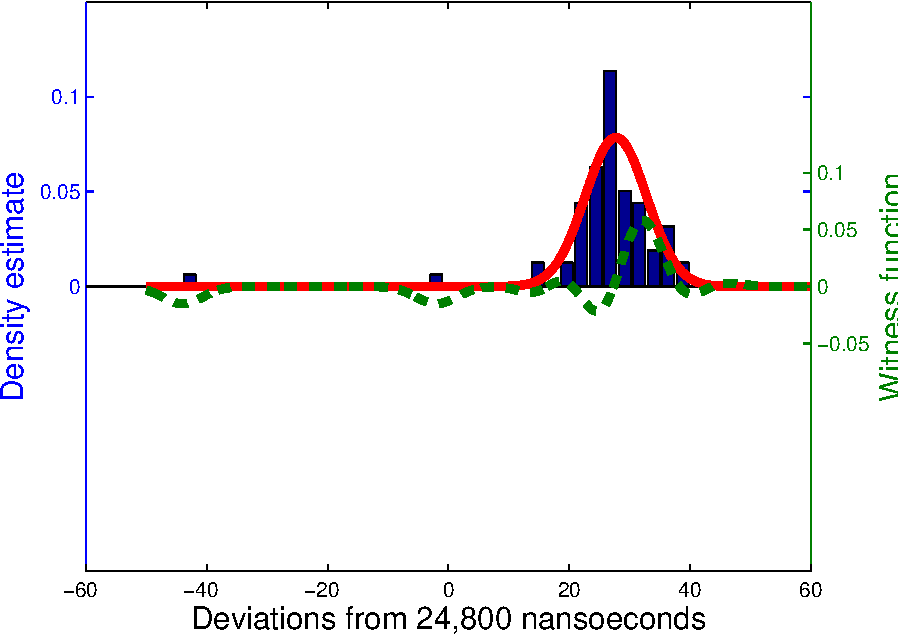
\includegraphics[width=0.32\columnwidth]{\criticismfigsdir/newcomb_witness_2}
\caption{
Left: Histogram of Simon Newcomb's speed of light measurements.
Middle: Histogram together with density estimate (red solid line) and MMD witness function (green dashed line).
Right: Histogram together with improved density estimate and witness function.
}
\label{fig:newcomb}
\end{figure}

To perform a MMD two sample test we sampled 1000 points from the fitted distribution, used the median heuristic to select a lengthscale and estimated the null distribution using 1000 bootstrap replications.
The estimated $p$-value of the test was less than 0.001 \ie a clear disparity between the model and data.
The data, fitted density estimate (the normal distribution) and witness function are shown in the middle of figure~\ref{fig:newcomb}.
The witness function has a trough at the centre of the data and peaks either side.
This indicates that the fitted model has placed too little mass in its centre and too much mass outside its centre.

This suggests that we should modify our model by either using a distribution with heavy tails or explicitly modelling the possibility of outliers which could have resulted in the variance being over-estimated.
However, to demonstrate some of the properties of the MMD statistic we make an unusual choice of fitting a Gaussian by maximum likelihood, but ignoring the two outliers in the data.
The new fitted density estimate (the normal distribution) and witness function of an MMD test are shown on the right of figure~\ref{fig:newcomb}.
The estimated $p$-value associated with the MMD two sample test is roughly 0.5, despite the fitted model being a very poor explanation of the outliers.
This demonstrates that the MMD test using a radial basis function kernel identifies dense discrepancies, rather than outliers.
However, methods that are not robust to outliers (\eg fitting a Gaussian by maximum likelihood) will likely show dense discrepancies that will be identified by the test.

\subsection{High dimensional data}

\label{sec:high_dim}

The interpretability of the witness functions comes from being equal to the difference of two kernel density estimates~\eqref{eq:witness-estimate}.
In high dimensional spaces, kernel density estimation is a very high variance procedure that can result in poor density estimates\fTBD{what is a classic citation?} which will destroy the interpretability of the method.
In response, we consider using dimensionality reduction techniques\fTBD{what is a classic citation?} before performing two sample tests.
Note however that the statistical test derived from the MMD still has high power in high dimensions \citep{Gretton2008-ik}.

To test how the MMD statistic can be used for high dimensional data we generated synthetic data using the following recipe.
5 points in a 10 dimensional space were drawn at random from a random 4 dimensional subspace\footnotemark.
\footnotetext{The details are not especially important; code for replication will be available upon publication}
Data was generated as isotropic Gaussian distributions centred on 4 of the 5 points.
Finally, data was centred on the fifth point drawn from an isotropic $t$-distribution with 2 degrees of freedom.
In sum, the data is a mixture of Gaussians and a $t$-distribution.

We then fit a mixture of Gaussians \citep[e.g.][]{McLachlan2004-qz} with 5 centres to the data and then generated samples from the fitted distribution in order to perform an MMD two sample test.
We reduced the dimensionality of the data using principal component analysis (PCA), selecting the first two principal components.
To ensure that the MMD test remains well calibrated we include the PCA dimensionality reduction within the bootstrap estimation of the null distribution.
The data and posterior predictive samples are plotted on the left of figure~\ref{fig:high_mog}.
While we can see that one cluster is different from the rest, it is difficult to assess by eye if these distributions are different --- due in part to the difficulty of plotting two sets of samples on top of each other.

\begin{figure}[ht]
\centering
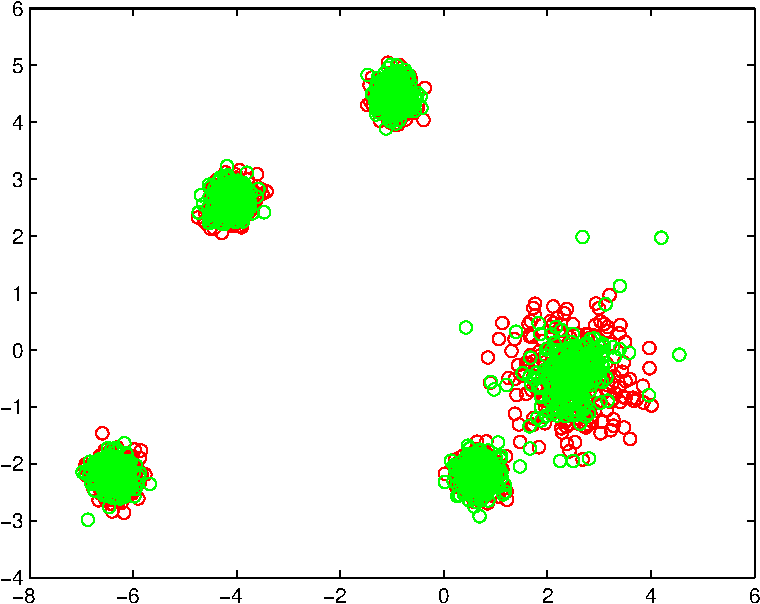
\includegraphics[width=0.3\columnwidth]{\criticismfigsdir/high_mog_pca}
\hspace{0.1\columnwidth}
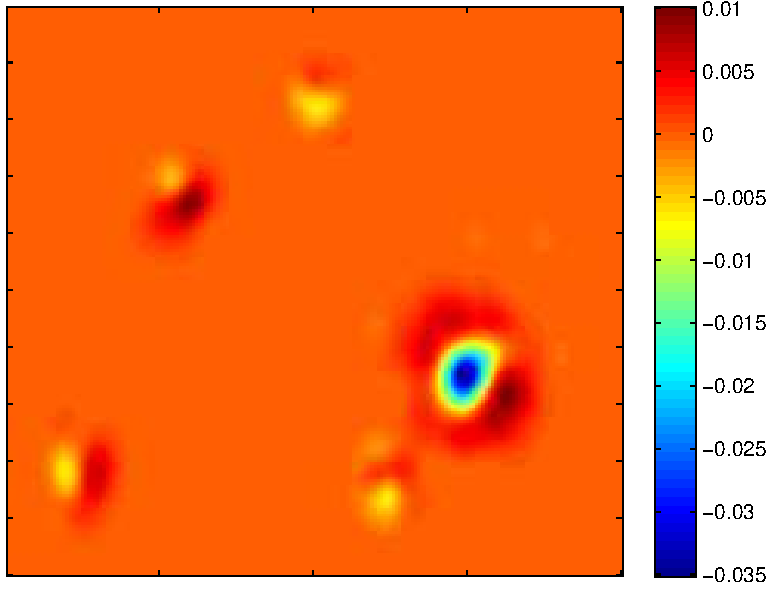
\includegraphics[width=0.31\columnwidth]{\criticismfigsdir/high_mog_witness}
\caption{
Left: PCA projection of synthetic high dimensional cluster data (green circles) and projection of samples from fitted model (red circles).
Right: Witness function of MMD two sample test. The erroneously fit cluster is clearly identified.
}
\label{fig:high_mog}
\end{figure}

Using the median heuristic to select a lengthscale results in a test that returns a $p$-value of 0.91, indicating that the test has not identified any discrepancies.
Indeed, the lengthscale chosen by this heuristic is $4.4$ which is of the order of the distances between clusters.
The test therefore is blind to discrepancies smaller than distances between clusters\footnotemark, and since the mixture of Gaussians has correctly identified the 5 centres and sizes of the mixture distribution, the test does not find any discrepancies.
\footnotetext{With enough data the test would eventually identify discrepancies on any scale --- however, the required amount of data can easily be very large}

However, taking the density estimate interpretation of the witness function more seriously suggests choosing lengthscales that result in the best density estimates.
We therefore selected a lengthscale by 5 fold cross validation using predictive likelihood of the kernel density estimate as the selection criterion.
With this lengthscale the MMD test returns a $p$-value of 0.05 and the witness function (right of figure~\ref{fig:high_mog}) clearly identifies the cluster that has been incorrectly modelled.

Presented with this discrepancy a statistical modeller might try a more flexible clustering model \citep[e.g.][]{Peel2000-pv, Iwata2012-yj} (a mixture of $t$-distributions would work on this example).
However, the $p$-value of the MMD statistic can also be made non-significant by fitting a mixture of 10 Gaussians.
We mention this as a reminder that the test proposed here does not attempt to falsify a class of models, it tests only whether or not the data could plausibly have been generated by a particular fitted model.

\section{Applications to real data and complex statistical models}

\subsection{What exactly do neural networks dream about?}

``To recognize shapes, first learn to generate images'' quoth Hinton \citep{Hinton2007-eo}.
Restricted Boltzmann Machine (RBM) pretraining of neural networks was shown by \cite{Hinton2006-yw} to learn a deep belief network (DBN) for the data \ie a generative model.
In agreement with this observation, as well as computing estimates of marginal likelihoods and testing errors, it has been standard to demonstrate the effectiveness of a neural network by generating samples from the distribution it has learned.

When trained on the MNIST handwritten digit data, samples from RBMs and DBNs certainly look like digits, but it is hard to detect any systematic anomalies purely by visual inspection.
We now use the kernel MMD two-sample test to investigate how faithfully RBMs and DBNs can capture the distribution over handwritten digits.

\subsubsection{RBMs mistake the identity of digits}

We trained an RBM with architecture $(784)\leftrightarrow(500)\leftrightarrow(10)$\footnotemark~using 15 epochs of persistent contrastive divergence PCD-15, a batch size of 20 and a learning rate of 0.1 (\ie we used the same settings as the code available at the deep learning tutorial \citep{deep-learning-tutorial}).
\footnotetext{That is, 784 input pixels and 10 indicators of the class label are connected to 500 hidden neurons.}
We generated 3000 independent samples from the learned generative model by initialising the network with a random training image and performing 1000 gibbs updates with the digit labels clamped\footnotemark~to generate each image (as in \eg \cite{Hinton2007-eo}).
\footnotetext{Without clamping the label neurons, the generative distribution is heavily biased towards certain digits.}

The top left of figure~\ref{fig:digits} shows twenty random samples\footnotemark~from this model.
\footnotetext{
Specifically these are the activations of the pixel neurons before sampling sampling binary values.
This is an attempt to be consistent with the grayscale input distribution of the images.
Analogous discrepancies would be discovered if we had instead sampled binary pixel values.}
They certainly look mostly like digits, but has the true distribution over digits been faithfully captured?
A priori the answer to this question is almost certainly no, but it is not immediately obvious how the learned distribution will deviate from the true distribution.

\begin{figure}[ht]
\centering
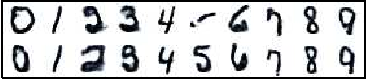
\includegraphics[width=0.48\columnwidth]{\criticismfigsdir/rbm_samples}
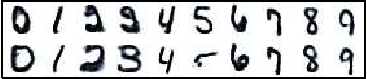
\includegraphics[width=0.48\columnwidth]{\criticismfigsdir/rbm_witness_troughs}
\\
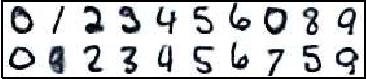
\includegraphics[width=0.48\columnwidth]{\criticismfigsdir/many_rbm_cond_witness_troughs}
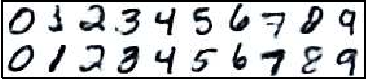
\includegraphics[width=0.48\columnwidth]{\criticismfigsdir/dbn_ft_cond_witness_troughs}
\\
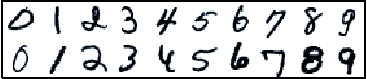
\includegraphics[width=0.48\columnwidth]{\criticismfigsdir/many_rbm_cond_witness_peaks}
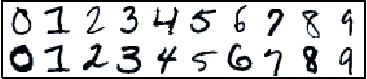
\includegraphics[width=0.48\columnwidth]{\criticismfigsdir/dbn_ft_cond_witness_peaks}
\caption{
Top left: Random samples from an RBM.
Top right: Troughs of the witness function for the RBM (digits that are over-represented by the model).
Middle left: Troughs of the witness function for samples from 1500 RBMs.
Middle right: Troughs of the witness function for the DBN.
Bottom left: Peaks (digits that are under-represented by the model) of the witness function for samples from 1500 RBMs.
Bottom right: Peaks of the witness function for the DBN.
}
\label{fig:digits}
\end{figure}

Since we generated digits from the class conditional distributions we compare each class separately.
However, for reference, the top plot of figure~\ref{fig:criticism:rbm_pca} displays the two dimensional PCA projection of MNIST digits (green circles) and samples from the RBM trained on this data (red crosses).
It is entirely clear that the RBM has not faithfully captured the distribution of the data it was trained on.
The situation is even worse when looking at the class conditional distributions of single digits.
The corresponding scatter plot for the distribution over the digit zero is shown in the bottom left plot of figure~\ref{fig:criticism:rbm_pca}.
To the right of this figure is the corresponding witness function estimate.
In this case it is easy to judge by eye where the discrepancies between model and data are most extreme without the witness function.
The usefulness of the test comes into play for more borderline situations demonstrated later.

\begin{figure}[ht]
  \begin{center}
  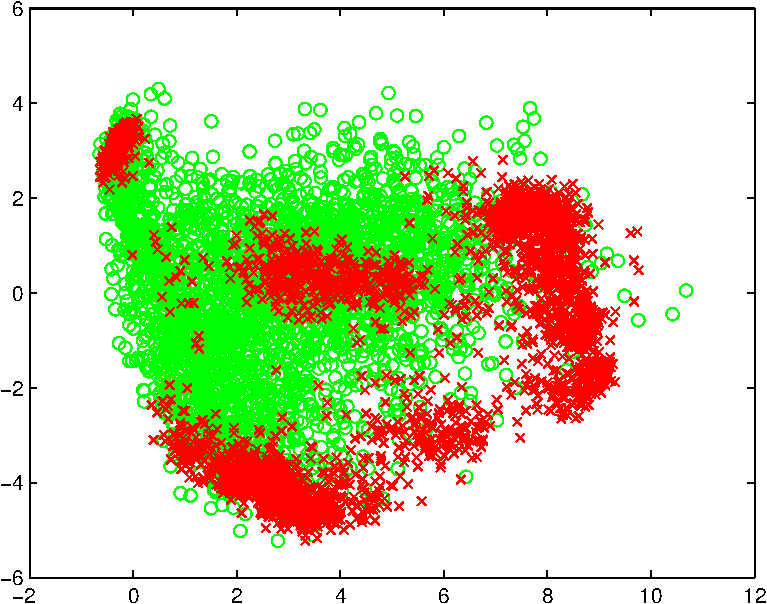
\includegraphics[width=0.4\columnwidth]{\criticismfigsdir/rbm_pca}
  \end{center}
  \begin{center}
  \begin{tabular}{cc}
    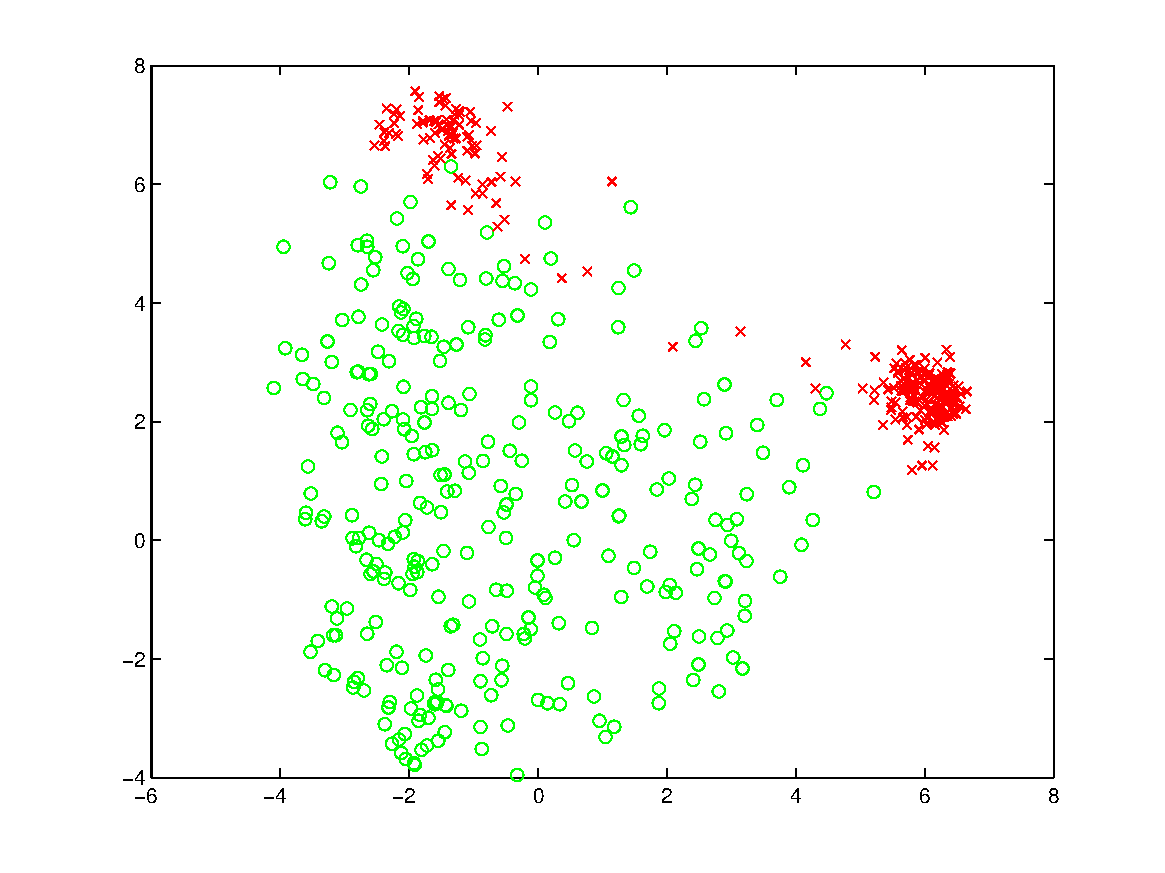
\includegraphics[width=0.4\columnwidth]{\criticismfigsdir/rbm_0_pca} & 
    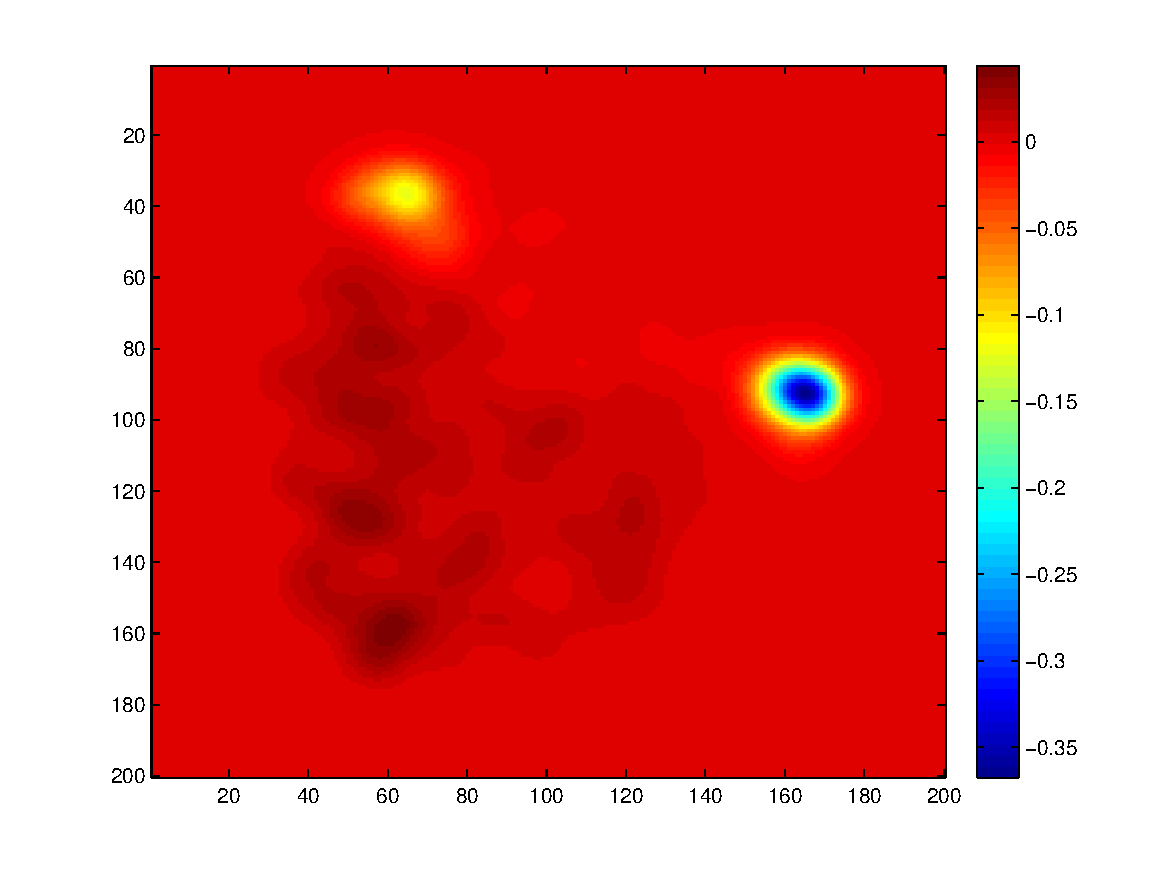
\includegraphics[width=0.4\columnwidth]{\criticismfigsdir/rbm_0_witness}
  \end{tabular}
  \end{center}
  \caption{Top: PCA projection of MNIST digits (green circles) and sample from a trained RBM (red crosses). These are certainly not from the same distribution. Left: Same as top plot but applied to the zero digit class conditional distribution. Right: Estimated witness function for left plot.}
  \label{fig:criticism:rbm_pca}
\end{figure}

Rather than show plots of the witness function for each digit we summarise the witness function by examples of digits closest to the peaks and troughs of the witness function (the witness function estimate is differentiable so we can find the peaks and troughs by gradient based optimisation).
We apply the MMD two-sample test to each class conditional distribution, using PCA to reduce to 2 dimensions and selecting the lengthscale via cross validation as in section~\ref{sec:high_dim}.

The top right box of figure~\ref{fig:digits} shows the digits closest to the two most extreme troughs\footnotemark~of the witness function for each class; the troughs indicate where the fitted distribution over-represents the distribution of true digits.
\footnotetext{
The exact ordering of the peaks and troughs is as follows.
We partition the space by grouping samples where the witness function has the same sign and gradient based optimisation of the witness function starting from each sample would reach the same peak or trough.
The contribution to the MMD from each of these groups is used to order the peaks and troughs.
}
The estimated $p$-value for all tests was less than 0.001.
The most obvious error with these digits is that the first 2 and 3 look quite similar.

To test that this was not just a poorly trained single RBM, we trained 1500 RBMs (with differently initialised pseudo random number generators) and generated one sample from each and performed the same tests.
The estimated $p$-values were again all less than 0.001 and the summaries of the troughs of the witness function are shown in the middle left box of figure~\ref{fig:digits}.
On the first toy data example we observed that the MMD statistic does not highlight outliers and therefore we can conclude that RBMs are making consistent mistakes \eg generating a 0 from the 7 distribution or a 5 when it should have been generating an 8.

\subsubsection{DBNs have nightmares about ghosts}

We now test the effectiveness of deep learning to represent the distribution of MNIST digits.
In particular, we fit a DBN with architecture $(784)\leftarrow(500)\leftarrow(500)\leftrightarrow(2000)\leftrightarrow(10)$ using RBM pre-training and a generative fine tuning algorithm described in \cite{Hinton2006-yw}.
Performing the same tests with 3000 samples results in estimated $p$-values of less than 0.001 except for the digit 4 (0.150) and digit 7 (0.010).
Summaries of the witness function troughs are shown in the middle right box of figure~\ref{fig:digits}.

The witness function no longer shows any class label mistakes (except perhaps for the digit 1 which looks very peculiar) but the 2, 3, 7 and 8 appear `ghosted' --- the digits fade in and out.
For comparison the bottom right box of figure~\ref{fig:digits} shows digits closest to the peaks of the witness function; there is no trace of ghosting.

Returning to the RBMs, we do not see ghosting either, but the digits nearest the witness function troughs are somewhat blurred (see bottom left box for comparison with peaks).
Assuming that the top level associative memory of the DBN also suffers from blurring, this will result in occasionally incorrect neurons in the second hidden layer on the DBN.
These incorrect bits will then propagate down the DBN resulting in spurious features in several visible neurons, resulting in ghosting.

\subsection{Testing non \iid data}
\label{sec:non_iid}

The test described so far applies when the model being tested has an \iid predictive distribution.
This is of course restrictive, so we now demonstrate how we can construct a test for a non \iid model based on the MMD statistic.
In particular we consider regression.

\subsubsection{A test of local heteroscedasticity and non-normality for regression}

We now assume that our data consists of pairs of inputs and outputs ${(x_i^\textrm{obs}, y_i^\textrm{obs})_{i=1\ldots n}}$.
A typical formulation of the problem of regression is to estimate the conditional distribution of the outputs given the inputs ${p(y\given x, \theta)}$.
This is consistent with assuming that input-output pairs are generated \iid from some distribution ${p(y, x \given \theta)}$, but conditioned on observing the particular input values ${(x_i^\textrm{obs})_{i=1\ldots n}}$.

Following this observation, we might consider generating data from the plug-in conditional distribution ${y_i^\textrm{rep} \dist p(y\given x_i^\textrm{obs}, \hat\theta)}$ and computing the empirical MMD estimate~\eqref{eq:MMD_b} between ${(x_i^\textrm{obs}, y_i^\textrm{obs})_{i=1\ldots n}}$ and ${(x_i^\textrm{obs}, y_i^\textrm{rep})_{i=1\ldots n}}$.
The only difference between this test and the MMD two sample test is that our data is generated from conditional distributions, rather than being \iid.
The null distribution of this statistic can be trivially estimated by sampling several sets of replicate data from the plug-in predictive distribution.

To demonstrate this test we apply it to 4 regression algorithms and 13 time series analysed in \cite{Lloyd2014-ABCD}.
In this work the authors compare several methods for constructing Gaussian process \citep[e.g.][]{Rasmussen2006-ml} regression models.
Example data sets are shown in figures~\ref{fig:SE-witness}~and~\ref{fig:ABCD-witness}.
While it is clear that simple smoothing methods will fail to capture all of the structure in the data, it is not clear a priori how much better the more advanced methods will fair.

To construct $p$-values we use held out data using the same split of training and testing data as the interpolation experiment in \cite{Lloyd2014-ABCD}.
Gaussian processes when applied to regression problems learn a joint distribution of all output values.
However, this joint distribution information is rarely used; typically only the pointwise conditional distributions ${p(y\given x_i^\textrm{obs}, \hat\theta)}$ are used which is consistent with the test proposed here.

Table~\ref{table:ABCD-p-values} shows a table of $p$-values for 13 data sets and 4 model construction methods.
The four methods are Gaussian process regression using a squared exponential kernel (SE), trend-cyclical-irregular models \citep[e.g.][]{lind2006basic} (TCI), spectral mixture kernels \citep{WilAda13} (SP) and the method proposed in \cite{Lloyd2014-ABCD} (ABCD).
Values in  bold indicate a positive discovery after a Benjamini--Hochberg \citep{Benjamini_undated-mh} procedure with a false discovery rate of 0.05 applied to each model construction method.
SE, TCI and SP have a very similar pattern of significant $p$-values whereas ABCD has fewer significant $p$-values.

\begin{table}[ht]
\center
\begin{tabular}{|c|c|c|c|c|}
\hline
Dataset & SE & TCI & SP & ABCD \\
\hline
Airline        & 0.36 & \bf{0.00} & 0.07 & 0.15 \\
Solar          & \bf{0.00} & \bf{0.00} & \bf{0.00} & 0.05 \\
Mauna          & 0.99 & 0.41 & 0.34 & 0.21 \\
Wheat          & \bf{0.00} & \bf{0.00} & \bf{0.00} & 0.19 \\
Temperature    & 0.54 & 0.83 & 0.68 & 0.75 \\
Internet       & \bf{0.00} & \bf{0.01} & 0.05 & \bf{0.01} \\
Call centre    & \bf{0.02} & \bf{0.00} & \bf{0.00} & 0.07 \\
Radio          & \bf{0.00} & \bf{0.00} & \bf{0.00} & \bf{0.00} \\
Gas production & \bf{0.00} & \bf{0.01} & \bf{0.01} & 0.11 \\
Sulphuric      & 0.29 & 0.38 & 0.34 & 0.52 \\
Unemployment   & \bf{0.00} & \bf{0.02} & \bf{0.00} & \bf{0.01} \\
Births         & \bf{0.00} & \bf{0.02} & \bf{0.00} & 0.12 \\
Wages          & \bf{0.00} & \bf{0.01} & \bf{0.01} & \bf{0.00} \\
\hline
\end{tabular}
\caption{Two sample test $p$-values applied to 13 time series and 4 regression algorithms.
Bold values indicate a positive discovery using a Benjamini--Hochberg procedure with a false discovery rate of 0.05 for each model construction method.}
\label{table:ABCD-p-values}
\end{table}

We now investigate the type of discrepancies found by this test by looking at the witness function (which can still be interpreted as the difference of kernel density estimates).
Figure~\ref{fig:SE-witness} shows the solar and gas production data sets, the posterior distribution of the SE fits to this data and the witness functions for the SE fit.
The solar witness function has a clear narrow peak, indicating that the data is more dense than expected by the fitted model in this region.
We can see that this has identified a region of low variability in the data \ie it has identified local heteroscedasticity not captured by the model.
Similar conclusions can be drawn about the gas production data and witness function.

\begin{figure}[ht]
\centering
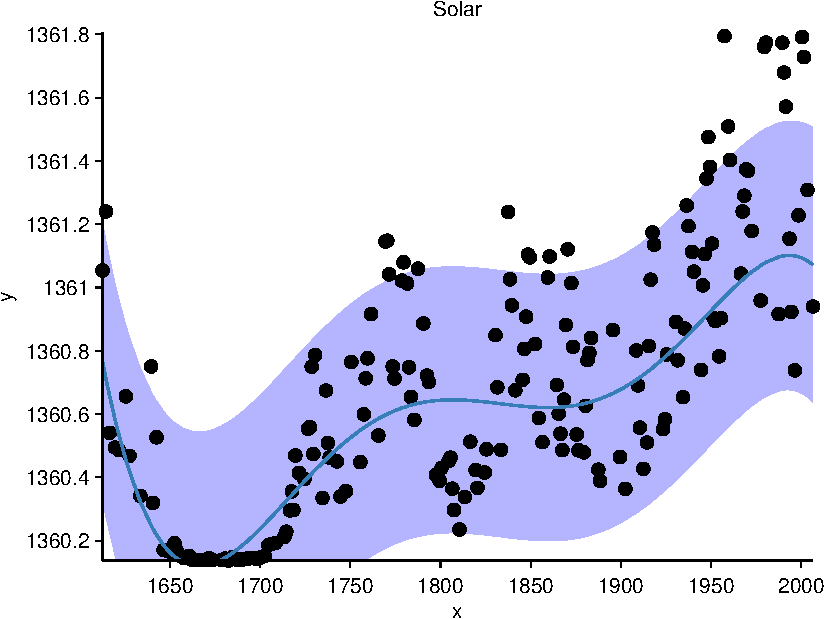
\includegraphics[width=0.22\columnwidth]{\criticismfigsdir/solar-data}
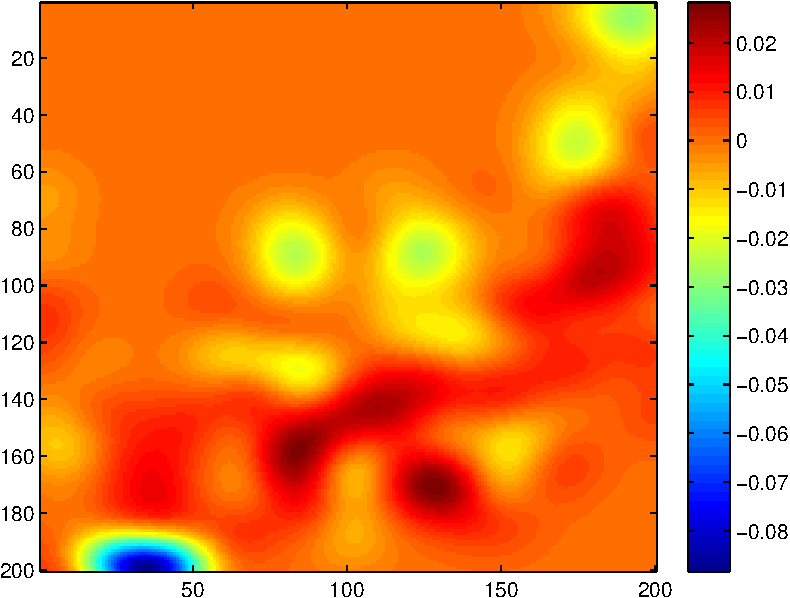
\includegraphics[width=0.22\columnwidth]{\criticismfigsdir/solar-witness}
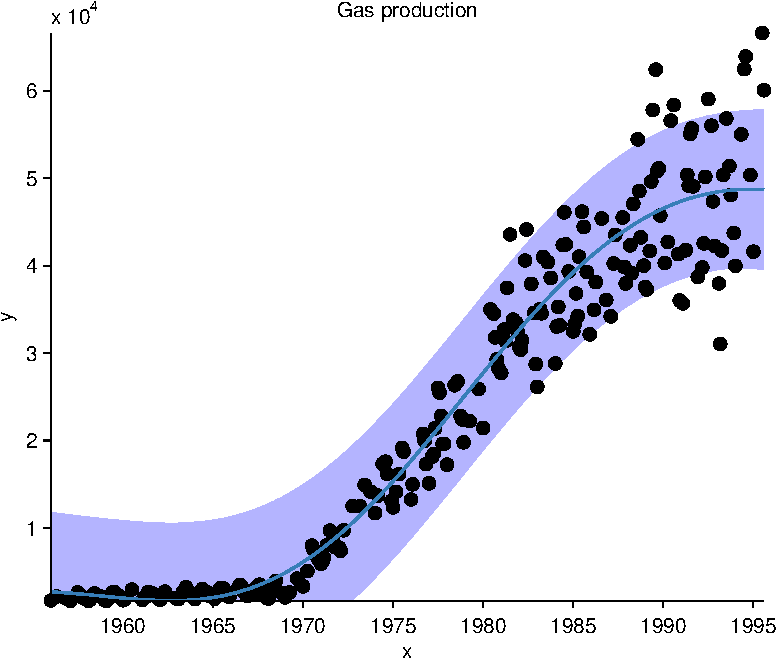
\includegraphics[width=0.22\columnwidth]{\criticismfigsdir/gas-data}
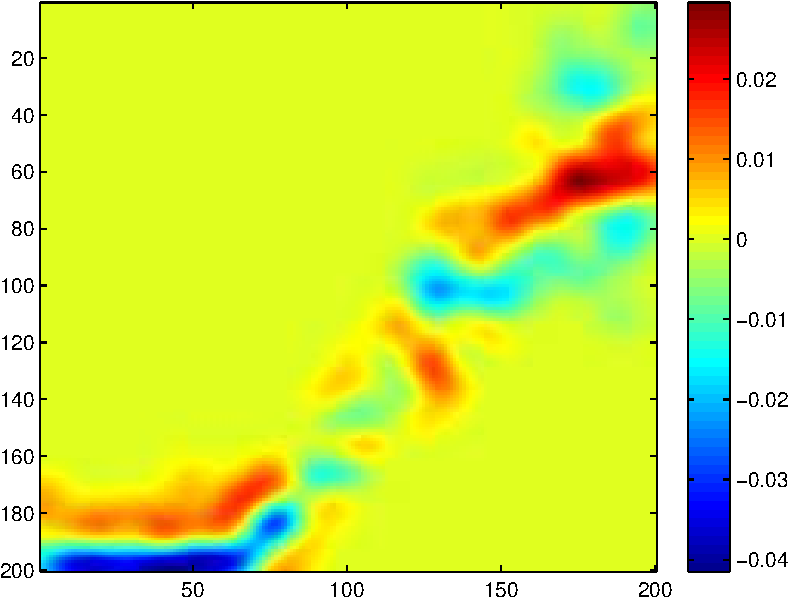
\includegraphics[width=0.22\columnwidth]{\criticismfigsdir/gas-witness}
\caption{
From left to right. Solar data with SE posterior. Witness function of SE fit to solar. Gas production data with SE posterior. Witness function of SE fit to gas production.
}
\label{fig:SE-witness}
\end{figure}

Of the four methods compared here, only ABCD is able to model heteroscedasticity, explaining why it is the only method with a substantially different set of significant $p$-values.
However, the procedure is still potentially failing to capture structure on four of the datasets.

Figure~\ref{fig:ABCD-witness} shows the unemployment and Internet data sets, the posterior distribution for the ABCD fits to the data and the witness functions of the ABCD fits.
The ABCD method has captured much of the structure in these data sets, making it difficult to visually identify discrepancies between model and data.
The witness function for unemployment shows peaks and troughs at similar values of the input $x$.
Comparing to the raw data we see that at these input values there are consistent outliers.
Since ABCD is based on Gaussianity assumptions these consistent outliers have caused the method to estimate a large variance in this region, when the true data is non-Gaussian.
There is also a similar pattern of peaks and troughs on the internet data suggesting that non-normality has again been detected.
Indeed, the data appears to have a strict lower bound which is inconsistent with Gaussianity.

\begin{figure}[ht]
\centering
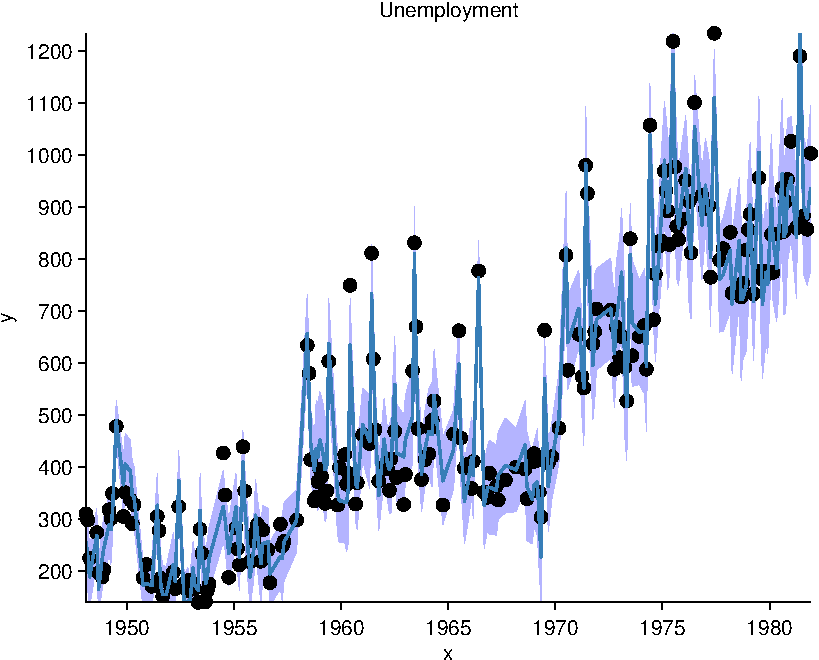
\includegraphics[width=0.22\columnwidth]{\criticismfigsdir/unemployment-data}
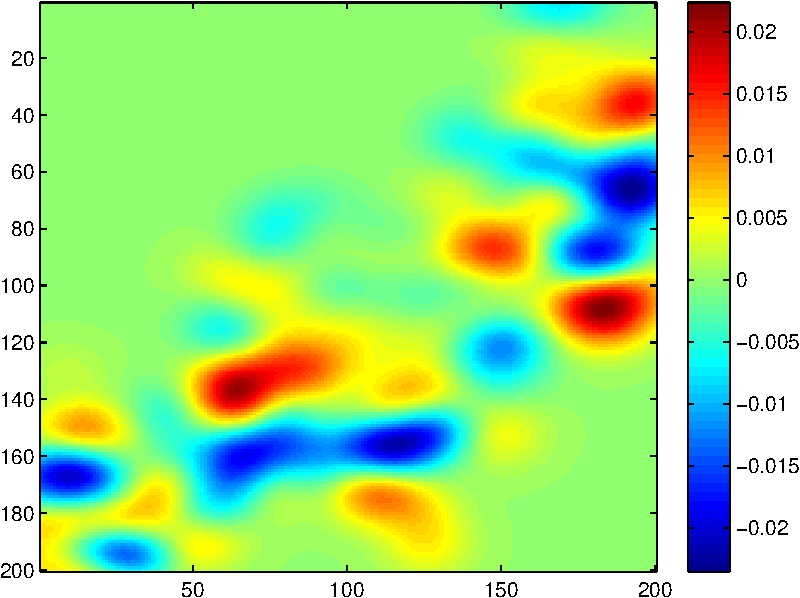
\includegraphics[width=0.22\columnwidth]{\criticismfigsdir/unemployment-witness}
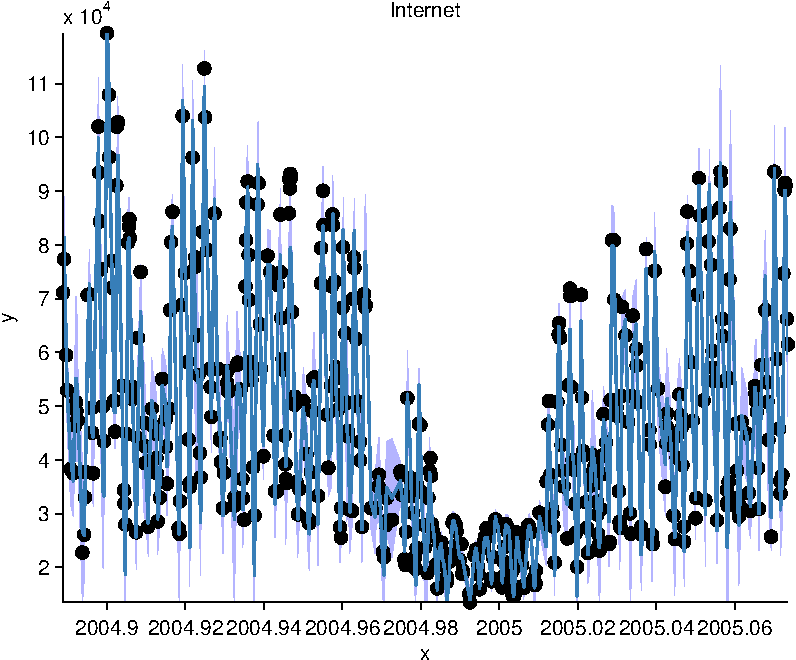
\includegraphics[width=0.22\columnwidth]{\criticismfigsdir/internet-data}
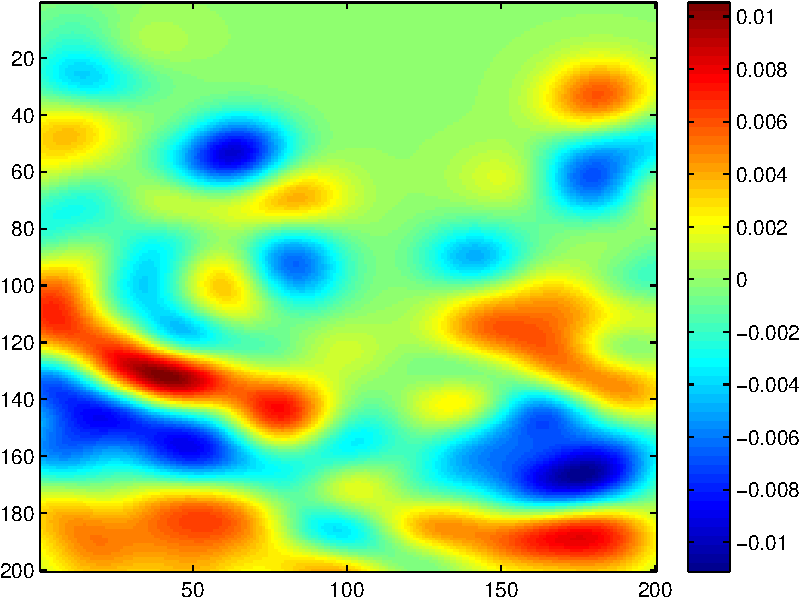
\includegraphics[width=0.22\columnwidth]{\criticismfigsdir/internet-witness}
\caption{
From left to right. Unemployment data with ABCD posterior. Witness function of ABCD fit to unemployment. Internet data with ABCD posterior. Witness function of ABCD fit to Internet.
}
\label{fig:ABCD-witness}
\end{figure}

\section{Further applied examples}

\TBD{Can we recreate any of Andrew Gelman's model criticism related ideas in a moderately objective manner.}

\section{Discussion of model criticism and related work}

\subsection{Are we criticising a particular model, or class of models?}

In section~\ref{sec:model-crit-general} we interpreted the differences between classical, Bayesian prior/posterior and plug-in $p$-values as corresponding to different null hypotheses and interpretations of the word `model'.
In particular the classical $p$-value tests a null hypothesis that the data could have been generated by a class of distributions (\eg all normal distributions) whereas all other $p$-values test a particular probability distribution.

Robins, van der Vaart \& Ventura \citep{Robins2000-oz} demonstrated that Bayesian and plug-in $p$-values are not classical $p$-values (frequentist $p$-values in their terminology) \ie they do not have a uniform distribution under the relevant null hypothesis.
However, this was presented as a failure of these methods; in particular they demonstrated that methods proposed by Bayarri \& Berger \citep{Bayarri1999-ty} based on posterior predictive $p$-values are asymptotically classical $p$-values.

This claimed inadequacy of posterior predictive $p$-values was rebutted \citep{Gelman2003-xx} and while their usefulness is becoming more accepted (see \eg introduction of \cite{Bayarri2007-cp}) it would appear there is still confusion on the subject \citep{Gelman2013-am}.
We hope that our interpretation of the differences between these methods as different null hypotheses --- appropriate in different circumstances --- sheds further light on the matter.

\subsection{Should we worry about using the same data for training and criticism?}

Plug-in and posterior predictive $p$-values test the null hypothesis that the observed data could have been generated by the fitted model or posterior predictive distribution.
In some situations it may be more appropriate to attempt to falsify the null hypothesis that future data will be generated by the plug-in or posterior predictive distribution.
As mentioned in section~\ref{sec:model-crit-general} this can be achieved by reserving a portion of the data to be used for model criticism alone, rather than fitting a model or updating a posterior on the full data.
Cross validation methods have also been investigated in this context \citep{Gelfand1992-ow, Gelfand1996-vy, Marshall2007-hd}.

\paragraph{Other methods for evaluating statistical models}

Other typical methods of model evaluation include estimating the predictive performance of the model, analyses of sensitivities to modelling parameters / priors, graphical tests, and estimates of model utility.
For a recent survey of Bayesian methods for model assessment, selection and comparison see \cite{Vehtari2012-oh} which phrases many techniques as estimates of the utility of a model.
For some discussion of sensitivity analysis and graphical model comparison see \citep[e.g.][]{Gelman2013-st}.

In this manuscript we have focused on methods that compare statistics of data with predictive distributions, ignoring parameters of the model.
The discrepancy measures of \cite{Gelman1996-ez} compute statistics of data and parameters; examples can be found in \cite{Gelman2013-st}.
O'Hagan \citep{OHagan2003-bc} also proposes a method and selectively reviews techniques for model criticism that also take model parameters into account.

In the spirit of scientific falsification \citep[e.g.][]{Popper2005-qq}, ideally all methods of assessing a model should be performed to gain confidence in any conclusions made.
Of course, when performing multiple hypothesis tests care must be taken in the intrepretation of individual $p$-values.

\section{Conclusions}

In this paper we have demonstrated an exploratory form of model criticism based on two sample tests using kernel maximum mean discrepancy.
In contrast to other methods for model criticism, the test analytically maximises over a broad class of statistics, automatically identifying the statistic which most demonstrates the discrepancy between the model and data.
We demonstrated how this method of model criticism can be applied to neural networks and Gaussian process regression and demonstrated the ways in which these models were misrepresenting the data they were trained on.

We have demonstrated how kernel MMD two sample tests can be applied to model criticism, but they can be applied to any aspect of statistical modelling where two sample tests are appropriate.
This includes for example, Geweke's tests of markov chain posterior sampler validity \citep{Geweke2004-yx} and tests of markov chain convergence \citep[e.g.][]{Cowles1996-qy}.

The two sample tests proposed in this paper naturally apply to \iid data and models, but model criticism techniques should of course apply to models with other symmetries (\eg exchangeable data, logitudinal data / time series, graphs, functions any many others).
We have demonstrated an adaptation of the kernel MMD test to regression models
However, it is unclear whether maximum mean discrepancy measures can be naturally extended to all of these classes; investigating such extensions would be a profitable area for future study.

In proposing a new method of model criticism we hope we have also exposed the machine learning community to a useful set of tools for diagnosing potential inadequacies of models.
On this note, we conclude with a question.
Do you know how the model you are currently working with most misrepresents the data it is attempting to model?

\section{Discussion and future work}

\subsection{What happened to statistical power?}

In this chapter we have discussed hypothesis tests and $p$-values but have not mentioned the statistical power of these tests.
\TBD{Define power}.
The prevailing view of model criticism is that it is an exploratory process that can be performed when no alternative models are currently being entertained.
In particular, \citet{OHagan2003-bc} writes
\begin{quotation}
Model criticism \dots is intended as an open-minded phase of investigation
to identify any problems with the model. Formulation of explicit alternatives
comes after the model criticism phase has identified some problems.
\end{quotation}
but also notes
\begin{quotation}
It is recognised that alternatives are at least loosely implicit
in any choice of model criticism tools, but the role of model criticism is
essentially exploratory.
\end{quotation}
It seems reasonable to make efforts to characterise the class of distributions against which a particular test has high power to understand the types of discrepancy the test is likely to identify.

\TBD{Read about and discuss the characterisation of alternative hypotheses for MMD.}

\subsection{Should we not just attempt to fit ever larger models?}

\TBD{Cite Gelman's view on ever larger models.}
If after completing a statistical analysis one as the resources (intellectual, computational, \etc) to attempt to fit a larger or more complex statistical model then one should do so.
However, at some point it will be infeasible to do so.
At this point it may be worthwhile to consider some form of model criticism procedure since they are typically easier to create and perform than the corresponding expanded inference problem.

\subsection{Perhaps a decision theoretic viewpoint will bring some rationality to the problem}

How might model criticism interact with, for example, the kernel search procedure?
Ideally any model criticism procedures should check for discrepancies that indicate the kernel search should continue considering larger kernels and for discrepancies that cannot be helped by fancier kernels \eg outliers.
Supposing that model criticism is very inexpensive, then after evaluating any kernel we are faced with the decision of whether or not to continue with the search, or go back to the research drawing board or stop and go to the pub.
How do we make this decision?
We need to estimate the utility of these actions.
We could estimate the utility of these actions using the inexpensive model criticism techniques using some reasoning system with experience of performing this estimation.
This reasoning system cannot be the model itself; it must be something outside the model - potentially a deep neural net or a human brain.
Whilst the only option is a human brain we should probably stick with producing model criticism techniques that tell us interesting things.
Perhaps a reasoning system, when being told how the statistical model is likely to be used could imagine all sorts of problems and then compute the expected consequences of these problems.
It uses this to decide which things to test.
I like this idea - it is kind of like playing devil's advocate - thinking of the most devious thing that could screw things up.
Devil's advocate model criticism.
This feels like it could go somewhere.

The best philosophy of statistical model criticism is still unclear, but what is certain is that it is often easy to do and may help and should therefore be done in almost all situations that involve statistical modelling.

\outbpdocument{
\bibliographystyle{plainnat}
\bibliography{references.bib}
}
